\subsection{Figure and Geometry 图形与几何}
\begin{paracol}{2}
Digits are the building blocks of numbers.
\switchcolumn
数都是由数字所组成的。
\end{paracol}
\begin{table}[!hbtp]
\centering
\begin{tabular}{|c|c|c|}
\hline
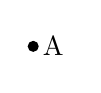
\begin{tikzpicture}[x=1cm,y=0.4cm]
    \fill (0,0) circle[radius=2pt];
    \draw (0,0) coordinate (a) node[right] {A};
\end{tikzpicture}
& Point 点& Point A 点A\\ \hline
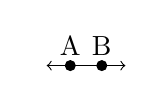
\begin{tikzpicture}[x=1cm,y=0.4cm]
	\draw (-0.5,0) coordinate (a0) node[left] {};
    \draw (-0.2,0) coordinate (a) node[above] {A};
    \draw (0.2,0) coordinate (b) node[above] {B};
    \draw (0.5,0) coordinate (b0) node {};
    \fill (-0.2,0) circle[radius=2pt];
     \fill (0.2,0) circle[radius=2pt];
     \draw[->](a) -- (a0);
    \path[draw] (a) -- (b);
    \draw[->] (b) -- (b0);
\end{tikzpicture}
& Line 直线& Line AB 直线AB\\ \hline
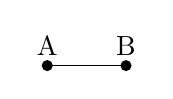
\begin{tikzpicture}[x=1cm,y=0.4cm]
    \draw (-0.5,0) coordinate (a) node[above] {A};
    \draw (0.5,0) coordinate (b) node[above] {B};
    \fill (-0.5,0) circle[radius=2pt];
     \fill (0.5,0) circle[radius=2pt];
    \path[draw] (a) -- (b);
\end{tikzpicture}
& Segment 线段& Segment AB 线段AB\\ \hline
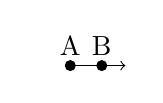
\begin{tikzpicture}[x=1cm,y=0.4cm]
	\draw (-0.5,0) coordinate (a0) node[left] {};
    \draw (-0.2,0) coordinate (a) node[above] {A};
    \draw (0.2,0) coordinate (b) node[above] {B};
    \draw (0.5,0) coordinate (b0) node {};
    \fill (-0.2,0) circle[radius=2pt];
     \fill (0.2,0) circle[radius=2pt];
    \path[draw] (a) -- (b);
    \draw[->] (b) -- (b0);
\end{tikzpicture}
& Ray 射线& Ray AB 射线AB\\ \hline
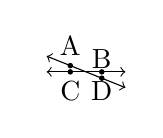
\begin{tikzpicture}[x=1cm,y=0.4cm]
	\draw (-0.5,0) coordinate (a0) node[left] {};
    \draw (-0.2,0) coordinate (a) node[below] {C};
    \draw (0.2,0) coordinate (b) node[below] {D};
    \draw (0.5,0) coordinate (b0) node {};
    \fill (-0.2,0) circle[radius=1pt];
     \fill (0.2,0) circle[radius=1pt];
     \draw[->](a) -- (a0);
    \path[draw] (a) -- (b);
    \draw[->] (b) -- (b0);
    \draw (-0.5,0.5) coordinate (aa0) node[left] {};
    \draw (-0.2,0.2) coordinate (aa) node[above] {A};
    \draw (0.2,-0.2) coordinate (bb) node[above] {B};
    \draw (0.5,-0.5) coordinate (bb0) node {};
    \fill (-0.2,0.2) circle[radius=1pt];
     \fill (0.2,-0.2) circle[radius=1pt];
     \draw[->](aa) -- (aa0);
    \path[draw] (aa) -- (bb);
    \draw[->] (bb) -- (bb0);
\end{tikzpicture}
& Intersecting lines 两线相交& Two lines meet in a point 两线有一个交点\\ \hline
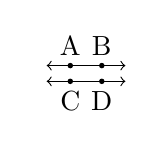
\begin{tikzpicture}[x=1cm,y=0.4cm]
	\draw (-0.5,0) coordinate (a0) node[left] {};
    \draw (-0.2,0) coordinate (a) node[below] {C};
    \draw (0.2,0) coordinate (b) node[below] {D};
    \draw (0.5,0) coordinate (b0) node {};
    \fill (-0.2,0) circle[radius=1pt];
     \fill (0.2,0) circle[radius=1pt];
     \draw[->](a) -- (a0);
    \path[draw] (a) -- (b);
    \draw[->] (b) -- (b0);
    \draw (-0.5,0.5) coordinate (aa0) node[left] {};
    \draw (-0.2,0.5) coordinate (aa) node[above] {A};
    \draw (0.2,0.5) coordinate (bb) node[above] {B};
    \draw (0.5,0.5) coordinate (bb0) node {};
    \fill (-0.2,0.5) circle[radius=1pt];
     \fill (0.2,0.5) circle[radius=1pt];
     \draw[->](aa) -- (aa0);
    \path[draw] (aa) -- (bb);
    \draw[->] (bb) -- (bb0);
\end{tikzpicture}
& Parallel lines 平行线& Line AB and CD never meet.  直线AB和CD不相交\\ \hline
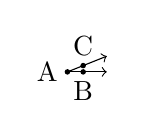
\begin{tikzpicture}[x=1cm,y=0.4cm]
    \draw (0,0) coordinate (a) node[left] {A};
    \draw (0.2,0) coordinate (b) node[below] {B};
    \draw (0.5,0) coordinate (b0) node {};
    \draw (0.2,0.2) coordinate (c) node[above] {C};
    \draw (0.5,0.5) coordinate (c0) node {};
    \fill (0,0) circle[radius=1pt];
     \fill (0.2,0) circle[radius=1pt];
      \fill (0.2,0.2) circle[radius=1pt];
    \path[draw] (a) -- (b);
    \draw[->] (b) -- (b0);
    \path[draw] (a) -- (c);
    \draw[->] (c) -- (c0);
\end{tikzpicture}
& Angle 角& Vertex: A, Sides: AB, AC 顶点:A,边:AB,AC\\ \hline
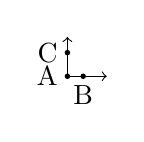
\begin{tikzpicture}[x=1cm,y=1cm]
    \draw (0,0) coordinate (a) node[left] {A};
    \draw (0.2,0) coordinate (b) node[below] {B};
    \draw (0.5,0) coordinate (b0) node {};
    \draw (0,0.3) coordinate (c) node[left] {C};
    \draw (0,0.5) coordinate (c0) node {};
    \fill (0,0) circle[radius=1pt];
     \fill (0.2,0) circle[radius=1pt];
      \fill (0,0.3) circle[radius=1pt];
    \path[draw] (a) -- (b);
    \draw[->] (b) -- (b0);
    \path[draw] (a) -- (c);
    \draw[->] (c) -- (c0);
\end{tikzpicture}
& Right Angle 直角& Right angle looks like a square. 直角两边互相垂直\\ \hline
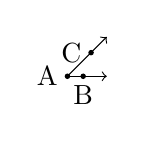
\begin{tikzpicture}[x=1cm,y=1cm]
    \draw (0,0) coordinate (a) node[left] {A};
    \draw (0.2,0) coordinate (b) node[below] {B};
    \draw (0.5,0) coordinate (b0) node {};
    \draw (0.3,0.3) coordinate (c) node[left] {C};
    \draw (0.5,0.5) coordinate (c0) node {};
    \fill (0,0) circle[radius=1pt];
     \fill (0.2,0) circle[radius=1pt];
      \fill (0.3,0.3) circle[radius=1pt];
    \path[draw] (a) -- (b);
    \draw[->] (b) -- (b0);
    \path[draw] (a) -- (c);
    \draw[->] (c) -- (c0);
\end{tikzpicture}
& Acute Angle 锐角& Acute angle is smaller than right angle. 锐角小于直角\\ \hline
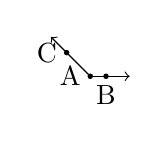
\begin{tikzpicture}[x=1cm,y=1cm]
    \draw (0,0) coordinate (a) node[left] {A};
    \draw (0.2,0) coordinate (b) node[below] {B};
    \draw (0.5,0) coordinate (b0) node {};
    \draw (-0.3,0.3) coordinate (c) node[left] {C};
    \draw (-0.5,0.5) coordinate (c0) node {};
    \fill (0,0) circle[radius=1pt];
     \fill (0.2,0) circle[radius=1pt];
      \fill (-0.3,0.3) circle[radius=1pt];
    \path[draw] (a) -- (b);
    \draw[->] (b) -- (b0);
    \path[draw] (a) -- (c);
    \draw[->] (c) -- (c0);
\end{tikzpicture}
& Obtuse Angle 钝角& Obtuse angle is larger than right angle. 钝角大于直角\\ \hline
\end{tabular}
\end{table}

\newpage
